\documentclass{article}
\usepackage{tikz, comment}
\usepackage{pifont}
\usepackage{fontspec}
\usetikzlibrary{arrows, decorations.markings, decorations.pathreplacing}
\begin{comment}
:Title: Not defined yet
:Tags: vertices;form;foci;curve
:Author: Prof.Hu Ji-shan, HKUST
:Slug: No name yet

Description Here.........
\end{comment}
\begin{document}\centering

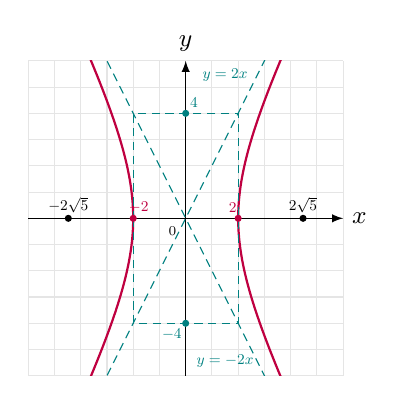
\begin{tikzpicture}[>=latex,xscale=.5/1.5, yscale=.5/1.5][font=\sf\small]

\draw[xstep=1cm,ystep=1cm,color=gray!20] (-6, -6) grid (6, 6);

\draw[->] ({-6}, 0) -- ({6}, 0)node[right] {\small $x$};
\draw[->] (0, {-6}) -- (0, {6})node[above] {\small $y$};

\clip[] (-6, -6) rectangle (6, 6);

\draw[purple, thick, samples=100, smooth, domain=-2:2, variable=\t]
plot ({sqrt(4)*(exp(\t)+exp(-\t))/2}, {sqrt(16)*(exp(\t)-exp(-\t))/2});

\draw[purple, thick, samples=100, smooth, domain=-2:2, variable=\t]
plot ({-sqrt(4)*(exp(\t)+exp(-\t))/2}, {sqrt(16)*(exp(\t)-exp(-\t))/2});

\draw[densely dashed, teal, samples=100, smooth, domain=-7:7, variable=\x]
plot ({\x}, {2*(\x)});

\draw[densely dashed, teal, samples=100, smooth, domain=-7:7, variable=\x]
plot ({\x}, {-2*(\x)});

\draw[densely dashed, teal] (-2,0)--++(0,-4)--++(4,0)--++(0, 8)--++(-4,0)--++(0,-4);

%\node[purple, xshift=-50, yshift=20, scale=0.6] at (0,0) {$y^2+2y+12x+25 = 0$};

\draw[black, fill] ({2*sqrt(5)}, {0}) circle(0.075*1.5)node[above, xshift=0, yshift=0, scale=0.6] {$2\sqrt{5}$};
\draw[black, fill] ({-2*sqrt(5)}, {0}) circle(0.075*1.5)node[above, xshift=0, yshift=0, scale=0.6] {$-2\sqrt{5}$};

\draw[purple, fill] ({2}, {0}) circle(0.075*1.5)node[above, xshift=-2, yshift=0, scale=0.6] {$2$};
\draw[purple, fill] ({-2}, {0}) circle(0.075*1.5)node[above, xshift=2, yshift=0, scale=0.6] {$-2$};

\draw[teal, fill] ({0}, {4}) circle(0.075*1.5)node[above, xshift=3, yshift=0, scale=0.6] {$4$};
\draw[teal, fill] ({0}, {-4}) circle(0.075*1.5)node[below, xshift=-5, yshift=0, scale=0.6] {$-4$};

\node[teal, above, xshift=0, yshift=0, scale=0.6] at ({1.5}, {5}) {$y = 2x$};
\node[teal, below, xshift=0, yshift=0, scale=0.6] at ({1.5}, {-5}) {$y = -2x$};

\node[scale=0.7] at (-0.2*2.5, -0.2*2.5) {\scriptsize$0$};

\end{tikzpicture}
\end{document}